%%%%%%%%%%%%%%%%%%%%%%%%%%%%%%%%%%%
%The LaTeX ARTICLE template for RSC journals was used
%Copyright The Royal Society of Chemistry 2016
%%%%%%%%%%%%%%%%%%%%%%%%%%%%%%%%%%%

\documentclass[twoside,twocolumn,9pt]{article}
\usepackage{extsizes}
\usepackage[super,sort&compress,comma]{natbib} 
\usepackage[version=3]{mhchem}
\usepackage[left=1.5cm, right=1.5cm, top=1.785cm, bottom=2.0cm]{geometry}
\usepackage{balance}
\usepackage{times,mathptmx}
\usepackage{sectsty}
\usepackage{graphicx} 
\usepackage{lastpage}
\usepackage[format=plain,justification=justified,singlelinecheck=false,font={stretch=1.125,small,sf},labelfont=bf,labelsep=space]{caption}
\usepackage{float}
\usepackage{fancyhdr}
\usepackage{fnpos}
\usepackage[english]{babel}
\usepackage{array}
\usepackage{droidsans}
\usepackage{charter}
\usepackage[T1]{fontenc}
\usepackage[usenames,dvipsnames]{xcolor}
\usepackage{setspace}
\usepackage[compact]{titlesec}
%%%Please don't disable any packages in the preamble, as this may cause the template to display incorrectly.%%%


%\usepackage{epstopdf}%This line makes .eps figures into .pdf - please comment out if not required.

\definecolor{cream}{RGB}{222,217,201}

\begin{document}

\pagestyle{fancy}
\thispagestyle{plain}
\fancypagestyle{plain}{

%%%HEADER%%%
\fancyhead[C]{\includegraphics[width=18.5cm]{head_foot/header_bar}}
\fancyhead[L]{\hspace{0cm}\vspace{1.5cm}\includegraphics[height=30pt]{head_foot/SM}}
\fancyhead[R]{\hspace{0cm}\vspace{1.7cm}\includegraphics[height=55pt]{head_foot/RSC_LOGO_CMYK}}
\renewcommand{\headrulewidth}{0pt}
}
%%%END OF HEADER%%%

%%%PAGE SETUP - Please do not change any commands within this section%%%
\makeFNbottom
\makeatletter
\renewcommand\LARGE{\@setfontsize\LARGE{15pt}{17}}
\renewcommand\Large{\@setfontsize\Large{12pt}{14}}
\renewcommand\large{\@setfontsize\large{10pt}{12}}
\renewcommand\footnotesize{\@setfontsize\footnotesize{7pt}{10}}
\makeatother

\renewcommand{\thefootnote}{\fnsymbol{footnote}}
\renewcommand\footnoterule{\vspace*{1pt}% 
\color{cream}\hrule width 3.5in height 0.4pt \color{black}\vspace*{5pt}} 
\setcounter{secnumdepth}{5}

\makeatletter 
\renewcommand\@biblabel[1]{#1}            
\renewcommand\@makefntext[1]% 
{\noindent\makebox[0pt][r]{\@thefnmark\,}#1}
\makeatother 
\renewcommand{\figurename}{\small{Fig.}~}
\sectionfont{\sffamily\Large}
\subsectionfont{\normalsize}
\subsubsectionfont{\bf}
\setstretch{1.125} %In particular, please do not alter this line.
\setlength{\skip\footins}{0.8cm}
\setlength{\footnotesep}{0.25cm}
\setlength{\jot}{10pt}
\titlespacing*{\section}{0pt}{4pt}{4pt}
\titlespacing*{\subsection}{0pt}{15pt}{1pt}
%%%END OF PAGE SETUP%%%

%%%FOOTER%%%
\fancyfoot{}
\fancyfoot[LO,RE]{\vspace{-7.1pt}\includegraphics[height=9pt]{head_foot/LF}}
\fancyfoot[CO]{\vspace{-7.1pt}\hspace{13.2cm}\includegraphics{head_foot/RF}}
\fancyfoot[CE]{\vspace{-7.2pt}\hspace{-14.2cm}\includegraphics{head_foot/RF}}
\fancyfoot[RO]{\footnotesize{\sffamily{1--\pageref{LastPage} ~\textbar  \hspace{2pt}\thepage}}}
\fancyfoot[LE]{\footnotesize{\sffamily{\thepage~\textbar\hspace{3.45cm} 1--\pageref{LastPage}}}}
\fancyhead{}
\renewcommand{\headrulewidth}{0pt} 
\renewcommand{\footrulewidth}{0pt}
\setlength{\arrayrulewidth}{1pt}
\setlength{\columnsep}{6.5mm}
\setlength\bibsep{1pt}
%%%END OF FOOTER%%%

%%%FIGURE SETUP - please do not change any commands within this section%%%
\makeatletter 
\newlength{\figrulesep} 
\setlength{\figrulesep}{0.5\textfloatsep} 

\newcommand{\topfigrule}{\vspace*{-1pt}% 
\noindent{\color{cream}\rule[-\figrulesep]{\columnwidth}{1.5pt}} }

\newcommand{\botfigrule}{\vspace*{-2pt}% 
\noindent{\color{cream}\rule[\figrulesep]{\columnwidth}{1.5pt}} }

\newcommand{\dblfigrule}{\vspace*{-1pt}% 
\noindent{\color{cream}\rule[-\figrulesep]{\textwidth}{1.5pt}} }

\makeatother
%%%END OF FIGURE SETUP%%%

%%%TITLE, AUTHORS AND ABSTRACT%%%
\twocolumn[
  \begin{@twocolumnfalse}
\vspace{3cm}
\sffamily
\begin{tabular}{m{4.5cm} p{13.5cm} }

\includegraphics{head_foot/DOI} & \noindent
\LARGE{\textbf{Evaporation of a microdroplet of a mixture of two liquids with different volatilities}}\\
\vspace{0.3cm} & \vspace{0.3cm} \\

 & \noindent\large{Maciej Kolwas, Daniel Jakubczyk,$^{\star}$ Tho DoDuc,$^{\ddag}$ and Justice Archer$\: ^{\mbox{\footnotesize \textsection}}$} \\

\includegraphics{head_foot/dates} & \noindent\normalsize{We've investigated fine details of evaporation of liquid mixture microdroplets. Several phenomena associated with their evaporation are identified, discussed and modelled analytically. We compare several essentially two-component mixtures, comprising of ethylene glycol (EG), diethylene glycol (DEG), triethylene glycol (TEG), glycerol and water. In this work we concentrate on effects of high-volatility components, as we studied the low-volatility impurities in [Jakubczyk \textit{et al., Acta Phys. Polon. A}, 2012, \textbf{122}, 709]. The more general findings are primarily exemplified by a practical case of DEG contaminated with water. Humid and dry ambient atmosphere is considered. In particular, we've observed a sigmoid transition of evaporation rate (surface change rate), which is known to be characteristic to evolution of population (amount) with limited resources. We showed that the transition itself can be comprehended with stationary evaporation model under instantaneous mixing condition. The condition was discussed and justified. The influence of composition of droplet and ambient atmosphere upon initial (pre-transition) stage of evaporation is considered in general manner. Three types of conditions are discussed concerning the presence of admixture in liquid and vapour phase (exemplified by DEG/water system): (i) dry liquid - dry atmosphere, (ii) wet liquid - dry atmosphere, and (iii) wet liquid - wet atmosphere. Case (i) has been successfully verified against the theoretical prediction. Case (ii) has required considering non-stationary liquid-in-liquid diffusion. Case (iii) led to a study of evaporation of a liquid mixture microdroplet with the more volatile component in equilibrium with its vapour.} \\
% The abstract should be a single paragraph which summarises the content of the article. Any references in the abstract should be written out in full \textit{e.g.}\ [Surname \textit{et al., Journal Title}, 2000, \textbf{35}, 3523].

\end{tabular}

 \end{@twocolumnfalse} \vspace{0.6cm}

  ]
%%%END OF TITLE, AUTHORS AND ABSTRACT%%%

%%%FONT SETUP - please do not change any commands within this section
\renewcommand*\rmdefault{bch}\normalfont\upshape
\rmfamily
\section*{}
\vspace{-1cm}


%%%FOOTNOTES%%%

\footnotetext{\textit{Institute of Physics, Polish Academy of Sciences, Warsaw, Poland; E-mail: jakub@ifpan.edu.pl}}

%Please use \dag to cite the ESI in the main text of the article.
%If you article does not have ESI please remove the the \dag symbol from the title and the footnotetext below.
\footnotetext{\ddag~Present address:}
%additional addresses can be cited as above using the lower-case letters, c, d, e... If all authors are from the same address, no letter is required

\footnotetext{\textsection~Present address:}
% Additional footnotes to the title and authors can be included \textit{e.g.}\ `Present address:' or `These authors contributed equally to this work' as above using the symbols: \ddag, \textsection, and \P. Please place the appropriate symbol next to the author's name and include a \texttt{\textbackslash footnotetext} entry in the the correct place in the list.}


%%%END OF FOOTNOTES%%%

%%%MAIN TEXT%%%%


\section{Introduction}
Evaporation of microdroplets is ubiquitous both in nature and technology and is associated with the most fundamental thermodynamic phenomena. Apart from pure thermodynamics, it belongs to the scope of physics of climate, aerosols and sprays, of microbiology and physiology. It is vital to technology of spray painting, crop spraying, medication administration, ink-jet printing, internal combustion engines and many others. Although  the physical principles of a droplet evaporation seem to have been established for over a century, the details still attract attention, as they turn out to play a crucial role at micro- and nanoscale. Many fundamental questions of chemical physics can be formed around these apparent details. Let's just mention the influence of the droplet surface phenomena and surface thermodynamics upon the processes in the droplet volume and the droplet volume evolution (evaporation). For microdroplets, evaporation takes place only at the surface - there is no boiling in microdroplets. Then, physics of surfaces (interfaces), decisively different from the physics in bulk, seems to be of fundamental importance. 

However, experimental studies of these phenomena in microdroplets of pure liquids encounter serious difficulties (see e.g. \cite{RoP} for a review). There is an issue of surface ageing and significant influence of impurities upon fine measurements. ``Pure'' liquids turn out to be never pure enough. Therefore, it seems reasonable to purposely study microdroplets of mixtures of well-defined composition. In particular, microdroplets of inhomogeneous mixtures (for instance suspensions), with very different behaviour of the surface in respect to the volume, can help to unravel the interactions between droplet's surface and volume and contribute to nanophysics of evaporation.

The results of droplet evaporation experiments seem to follow rather simple rules (e.g. the radius-square law - the linear temporal evolution of droplet surface area), while theoretical description and modelling calls upon complex, non-linear, multi-parameter formulas. Thus, in this work we start from experimental results and make phenomenological observations first. Then we try to explain the observed effects with simplest possible models. We concentrate on the mutual influence of two liquids in a mixture upon the droplet evaporation, trying to address the effect of surface versus volume phenomena and sigmoid transition. We limit the analysis to the condition of ideal mixing and thus carefully avoid azeotropes. We used a hygroscopic liquid (diethylene glycol) contaminated with water and in contact with dry or humid atmosphere, as a realistic mixture model. We analysed the impact of non-volatile and low-volatility impurities in \cite{Acta}. In this work we study the effect of high-volatility impurities. 

\section{Experimental methods}
We studied evaporation of single, free droplets with non-contact techniques. The details of our experimental setup can be found in \cite{weightvsscatt,Smigacz}, while its application was demonstrated e.g. in \cite{Hi-precission,HK-soft_matter,RoP,vs_molecular_mass,Archer}. The droplet was levitating in an electrodynamic quadrupole trap (see e.g. \cite{Paul} for the fundamentals and \cite{Knoop,Major} for a review of implementations)  and the trap was kept in a snugly fitting climatic chamber with well controlled (and stabilised) temperature profile. Such combination of the levitator and the chamber ensures high droplet sphericity and absence of both convection in the chamber atmosphere and vortices in the droplet. For the purpose of electrodynamic levitation, droplets must be electrically charged. Thus, only liquids with non-negligible polarity can be used. Individual droplets were injected into the trap with the droplet-on-demand injector (compare \cite{Wriedt}). The droplets were charged on emerging from the injector nozzle in the external field of the trap, without additional charger.

\begin{figure}[htb]
 \centering
  \rotatebox{-90}{\includegraphics[width=6.3cm]{setupmixed.eps}}
 \caption{Experimental setup - schematic drawing superimposed on a view of the complete chamber.}
 \label{setup4mixed}
\end{figure}

The chamber was purged and filled with gaseous nitrogen obtained from liquid nitrogen in order to ensure very low humidity.
We used two lots of diethylene glycol (DEG; Fluka, BioUltra): 99.9 and 99.99 GC area \%. It must be underlined, that the later was, according to lot data provided by the manufacturer, of exceptional purity. Several DEG samples were additionally contaminated (mostly) with water via exposure to ambient air.
We also used ethylene glycol (EG; Riedl-de {Ha\"{e}n}, Spectranal), 99.8 GC area \%, triethylene glycol (TEG; Fluka, BioUltra, anhydrous), 99.96 GC area \% and glycerol (Chempur, anhydrous, pure p.a.), 99.5 \%.

The evolution of the droplet radius was studied with a variant of static (elastic) light scattering method (Mie Scattering Look-up Table Method), which we developed (see \cite{Smigacz} and references therein). It belongs to the group of interferometric methods and thus can provide ultimate accuracy. Making use of two laser beams of different colours and perpendicular polarisations we were able to measure radius with up to $\pm 10$~nm accuracy. 

\section{Evaporation of a microdroplet of hygroscopic liquid}
In fine thermodynamic measurements of evaporating microdroplets a persistent problem of impurities arises. The concentration of impurities changes dramatically during the evolution: increases for low-volatility impurities and decreases for these highly volatile. In both cases the evaporation scenario is affected substantially enough to render finer thermodynamic measurements inconclusive.

The hygroscopic liquids make a particularly important case, being easily contaminated with high-volatility liquid - water. Water vapour is omnipresent and many materials - plastics in particular - contain a surprisingly high amount of water. Extreme care must be taken to keep hygroscopic material under study dry.

\begin{figure}[htb]
 %\centering
 \rotatebox{-90}{\includegraphics[width=6.5cm]{2aaprim.eps}}
 \caption{Examples of evolutions (surface change rate) of DEG microdroplets corresponding to different droplet and atmosphere compositions: traces in shades of green - pure DEG in dry N$_2$ atmosphere; traces in shades of blue - DEG contaminated with water in (nearly) dry N$_2$ atmosphere; traces in shades of grey - DEG contaminated with water in humid N$_2$ atmosphere. Each trace is labelled with the initial droplet radius. Theoretical prediction of evaporation of pure DEG in dry atmosphere shown with red dashed line. The grey band corresponds to prediction accuracy defined by the used parameters: vapour pressure \cite{MEG}, and diffusion coefficient from \cite{Lugg}). The observed rapid evolutions slow-downs are caused by non-volatile impurities. The full evolution of the largest droplet is shown in the inset.}
 \label{2aaprim}
\end{figure}

A selection of experimentally obtained evolutions of DEG (a highly hygroscopic liquid) microdroplets evaporating under diverse humidity/purity conditions are shown in figure \ref{2aaprim} in a form of surface change rate. Using such an observable facilitates studying multicomponent droplets, as for evaporation of pure component droplet, surface change rate is perfectly level. Since the derivative is sensitive even to minute signal modifications, any deviation from the radius-square law is plainly visible.

Each trace corresponds to a different initial droplet radius (shown in the colour of the line). Three groups of traces can be distinguished, and they are drawn in shades of green, blue and grey respectively.

Green curves correspond to the purest DEG and the most dry nitrogen atmosphere. The red, level line corresponds to the predicted stationary evaporation rate of ideally pure DEG (discussed further on; the thermodynamic parameters were taken from \cite{DEG, Lugg}) and the grey shaded region corresponds to prediction error limit. The beginning of evaporation - lowest concentration of  impurities - coincides with the predicted value well and it does not depend on the initial droplet radius. The presence of low-volatility impurities manifests itself as sigmoidal shape of the evolution curve with a gentle slope before and after the rapid transition. While the gentle slope can be intuitively accepted (compare the discussion we presented in \cite{Acta}), the rapid transition in evaporation rate seems counter-intuitive, since the concentration of impurities grows steadily in time. This characteristic sigmoid transition, associated with the evolution of population (amount) with limited resources, is encountered for all non-azeotropic mixtures and, as a matter of fact, greatly facilitates distillation. It can be well illustrated with the evolution of a EG-DEG (liquid-liquid) mixture droplet compared to single component droplet evolutions presented in figure \ref{2liquids}. We discuss the physics of this rapid transition, using the notion of stationary process only, in subsection \ref{stationary->sigmoid}.

However, the evolutions corresponding to DEG contaminated with water or/and in non-dry atmosphere, presented in figure \ref{2aaprim}, exhibit additional features. Apart from steeper initial slopes they also seem to depend on the initial droplet size. There are two groups of traces corresponding to non-pure/non-dry conditions. The traces presented in shades of blue correspond to evolutions faster then that of pure DEG, while the traces presented in shades of grey correspond to those that are slower.

In subsection \ref{liquid-liquid} we show that the former dependence can be reproduced by taking into account the non-stationary liquid-in-liquid diffusion in the droplet, governing the evaporation rate. In subsection \ref{in-equilibrium} we demonstrate that the latter dependence requires considering the phase equilibrium of the more volatile component. 

\begin{figure}[htb]
 \centering
 \rotatebox{-90}{\includegraphics[width=6.5cm]{EGDEG2aaprim.eps}}
 \caption{Red dots represent the evolution of a microdroplet of a EG-DEG mixture. The evaporation rate - surface change rate - decreases from that corresponding to pure EG (green dots) to that of pure DEG (blue dots). The black sigmoidal line represents the data fit with formula \ref{adota}. The temporal scales of these evolutions are visualised/compared in the inset.}
 \label{2liquids}
\end{figure}

\subsection{Sigmoid evolution of 2-component droplet evaporation rate} \label{stationary->sigmoid}
First, we shall introduce a simple description of the liquid mixture droplet stationary evaporation. We shall use classical vapour-in-gas diffusion equations limiting ourselves to the terms pertaining to the observed phenomena.

In case of evaporation of a multi-component droplet, the Raoult's law must be invoked. It is convenient then to express the vapour flux in terms of amount (moles) rather than of mass. Under the condition of instantaneous mixing, transport of a component $i$ from a microdroplet steadily evaporating into an atmosphere void of $i$-th component vapour can be rendered as  (compare e.g. \cite{Pruppacher} p. 504):
\begin{equation}
  \frac{dn_i}{dt} = -4\pi a D_i\rho_{{\rm sat},i} \frac{n_i}{\sum\limits_{i} n_i} \mbox{~,}
  \label{i-th_component}
\end{equation}
where $a$ is the droplet radius, while $n_i$, $D_i$ and $\rho_{{\rm sat},i}$ are the $i$-th component amount, vapour-in-gas diffusion coefficient and saturated vapour molar concentration. The Raoult's law is applied here in its equilibrium form (compare derivation of K\:{o}hler equations in \cite{Pruppacher} (p.172)) for the lack of a better analytical form. For a microdroplet, the effects of surface tension (described with Kelvin term) are negligible. Further on, for relatively slow evaporation, evaporative cooling can also be neglected.

Now, for the sake of analysis of data from figures \ref{2aaprim} - \ref{kinks}, we consider a two-liquid-component droplet evaporation, for which component 1 is much more volatile than 2. If we introduce a measure of their relative volatility as
\begin{equation}
\kappa := \frac{D_2\rho_{{\rm sat},2}}{D_1\rho_{{\rm sat},1}} \mbox{~, ~then ~$\kappa  \ll 1$~.}
\label{volatility}
\end{equation}
For example, in case of DEG/H$_2$O mixture, $\kappa \sim 10^{-4}$. 

In the considered cases, the assumption of instantaneous mixing can also be well justified. By invoking Einstein's relation \cite{Einstein1907} for 3-dimensional diffusion (see e.g. \cite{Keffer}) we can bind the characteristic length - the droplet radius $a$ - with the characteristic time of diffusion $\tau$:
\begin{equation}
\tau = \frac{a^2}{6D_{12}} \mbox{~,} \label{Einstein_diffusion}
\end{equation}
where $D_{12}$ is the liquid phase mutual diffusion coefficient of components 1 and 2. For example, for DEG/H$_2$O mixture, $D_{12} \simeq 10^{-9}$~m$^2$/s (see e.g. \cite{Wang_glycols_diffusion}), while for EG/DEG mixture $D_{12} \simeq 6 \times 10^{-11}$~m$^2$/s (see e.g.\cite{Mitchel}). Then, for a 10~$\mu$m-droplet, $\tau \simeq 0.02$~s and  0.3~s respectively, which is much less than the observed sigmoid transition times in figures  \ref{2aaprim} - \ref{kinks}.

Obviously, the preponderance of a component defines the total evaporation rate:
\begin{equation}
\frac{dn}{dt}=\frac{dn_1}{dt}+\frac{dn_2}{dt} \rightarrow
\begin{cases}
\mbox{fast:~} -4\pi a D_1\rho_{{\rm sat},1} \mbox{~,~} n_1 \gg n_2 \\
\mbox{slow:~} -4\pi a D_2\rho_{{\rm sat},2} \mbox{~,~} n_2 \gg n_1
\end{cases} \mbox{.}
\label{two_levels}
\end{equation}
However, the transition between the two evaporation rate levels is not obvious. From the symmetry of the problem, we expect that the rapid transition occurs around $dn_1/dt=dn_2/dt$. Interestingly, in view of condition \ref{volatility}, it follows from equation set \ref{i-th_component}, that 
\begin{equation}
\frac{dn_1}{dt}=\frac{dn_2}{dt} \mbox{~~implies~~} n_2 \gg n_1 \mbox{~.}
\label{equal_rates}
\end{equation}
It must be kept in mind, that this condition is not equivalent to condition \ref{two_levels}-slow.

Equation set \ref{i-th_component} yields an interesting first integral (constant of motion or conservation law):
\begin{equation}
\left[\frac{n_2(t)}{n_{2}(0)}\right]^{D_1\rho_{{\rm sat},1}}=\left[\frac{n_1(t)}{n_{1}(0)}\right]^{D_2\rho_{{\rm sat},2}} \mbox{~,}
\label{1st_integral}
\end{equation}
where $n_{1}(0)$ and $n_{2}(0)$ are the initial component amounts. This conservation law, analogue to Gibbs-Duhem equation, binds the relative amounts of components in liquid phase by means of their properties in gaseous phase. From \ref{i-th_component}, \ref{volatility} (definition) and \ref{1st_integral} follows:
\begin{align}
\frac{dn}{dt} & = \frac{dn_1}{dt}\left[ 1+\dfrac{n_{2}(0)}{n_{1}(0)}n_1^{\kappa - 1} \kappa \right]= \nonumber\\
& =-4\pi a \left[ \frac{D_1\rho_{{\rm sat},1}}{1+\dfrac{n_{2}(0)}{n_{1}(0)^{\kappa}}n_1^{\kappa - 1}} + \dfrac{D_2\rho_{{\rm sat},2}}{1+\dfrac{n_{1}(0)^{\kappa}}{n_{2}(0)}n_1^{-\kappa +1}} \right] \mbox{.}
\label{n1_a}
\end{align}
Making use of conditions \ref{volatility} and \ref{equal_rates} enables a significant simplification:
\begin{equation}
\frac{dn_1}{dt} = -4\pi a \left[ D_1\rho_{{\rm sat},1}\frac{n_1}{n_{2}(0)} + D_2\rho_{{\rm sat},2} \right] \mbox{.}
\label{simplified}
\end{equation}

\begin{figure}[htb]
 \centering
\rotatebox{-90}{\includegraphics[width=6.5cm]{kinks.eps}}
 \caption{Temporal evolutions of the square of droplet radius (proportional to the droplet surface area) for diverse liquid-liquid mixtures. Evolutions in different time-scales shown in separate panels. It is worth noticing that evaporation of a component seems to obey the radius-square-law. Middle panel: the evolution of single-component DEG droplet is shown for comparison. Transitions to level regions due to presence of low-volatility impurities are shown only for DEG and EG+DEG evolutions in middle panel.}
 \label{kinks}
\end{figure}
Now, from figure \ref{kinks} it can be noticed, that the transition in evaporation rate is relatively short-lasting. Therefore, in view of condition \ref{equal_rates}, it can be assumed that the mixture (droplet) total molar concentration $c_L$ is constant during the transition. However, in general, for ideal mixing
\begin{equation}
c_L = c_1 \frac{n_1}{n_1+n_2} + c_2 \frac{n_2}{n_1+n_2} \mbox{~,}
\label{c_L}
\end{equation}
where $c_i$ is the molar concentration of pure $i$-th component.
Then, the amount of matter in the droplet can be simply expressed as
\begin{equation}
\frac{4}{3}\pi a^3 c_L = n  \mbox{~.}
\label{amount}
\end{equation}
Using conditions \ref{volatility} and \ref{equal_rates} and equation \ref{1st_integral} it can be further approximated as:
\begin{equation}
\frac{4}{3}\pi a^3 c_2 \approx n_{2}(0)  \mbox{~.}
\label{a}
\end{equation}
Substituting \ref{a} into \ref{simplified} yields an ordinary differential equation for $n_1$ in the form of
\begin{equation}
\frac{dn_1}{dt} = -\alpha n_1 + \beta  \mbox{~,}
\label{n1}
\end{equation}
where
\begin{equation*}
\alpha = \zeta D_1 \rho_1 n_{2}(0)^{-2/3} \mbox{~,~~} 
\beta = \zeta D_2 \rho_2 n_{2}(0)^{1/3} \mbox{~,}
\end{equation*}
\begin{equation*}
\zeta = 4\pi \left( \frac{3}{4\pi c_2} \right) ^{1/3} \mbox{.}
\end{equation*}
The solution in general form is
\begin{equation}
n_1 = - \frac{\beta}{\alpha} + \left[ n_{1}(0) - \frac{\beta}{\alpha} \right] \exp \left( -\alpha t \right) \mbox{~,}
\end{equation}
where
\begin{equation*}
\frac{\beta}{\alpha} = \frac{D_2\rho_2}{D_1\rho_1} n_{2}(0)
\end{equation*}
In view of condition \ref{volatility}, $\beta / \alpha$ can be neglected (for DEG/H$_2$O mixture it is $\sim 10^{-12}$ mole) and the evolution of $n_1$ takes a form of single-exponential decay
\begin{equation}
n_1 =  n_{1}(0) \exp \left( -\alpha t \right) \mbox{~,}
\label{decay}
\end{equation}
as expected. It follows from \ref{amount} that
\begin{equation}
a\frac{da}{dt} = \frac{1}{4\pi ac_L} \frac{dn}{dt}  \mbox{~.}
\label{adota}
\end{equation}
Then, from \ref{adota} and \ref{n1_a} the analytical formula describing the transition can be obtained:
\begin{equation}
\frac{dS}{dt} = -\frac{8\pi}{c_L} \left[ \frac{D_1\rho_{{\rm sat},1}}{1+\dfrac{n_{2}(0)}{n_{1}(0)}\exp\left(\alpha t\right)} + \dfrac{D_2\rho_{{\rm sat},2}}{1+\dfrac{n_{1}(0)}{n_{2}(0)}\exp\left(-\alpha t\right)} \right] \mbox{~,}
\label{sigmoidal}
\end{equation}
where $S$ is the droplet surface area. We demonstrate it in figure \ref{2liquids} by fitting the evolution of an EG+DEG microdroplet with this formula. The above reasoning, in general, also explains the sigmoid transitions observed in figure \ref{2aaprim} (action of low-volatility impurities). However, the features observed before these transitions require further analysis.

\subsection{Influence of the liquid-in-liquid diffusion} \label{liquid-liquid}
Diffusion of a component in liquid phase is much slower than in gas phase. For instance, the diffusion coefficients of DEG in water and in air differ by over 4 orders of magnitude. Since the flux of an evaporating component is continuous across gas-liquid interface, certain stages of evaporation of a droplet of liquid mixture are largely controlled by the liquid-in-liquid diffusion. First of all, in case of a microdroplet, the process is non-stationary due to limited amount of the diffusing/evaporating component. In order to describe the transitory effects observed experimentally for evaporating microdroplets of two-liquid compounds, Fick's second law of diffusion must be invoked in spherical coordinates. However, this partial differential equations can not be sensibly solved for the boundary conditions imposed by the problem symmetry and, in consequence, the evolution of the component concentration distribution can not be found analytically. Nevertheless, the problem can be circumvented, since we already know from the corollary of formula \ref{Einstein_diffusion}, that the concentration distribution is nearly homogeneous in the studied cases. Then the observed effects can be modelled by utilizing the flux density notion:
\begin{equation}
\frac{\partial c_1}{\partial t} + \nabla _r j_1(r,t) = 0 \mbox{~,}
\label{II_Fick}
\end{equation}
where $c_1$ is the molar concentration and $j_1$ is the flux density of high-volatility component in low-volatility component in liquid phase.
At the surface, the flux density in liquid and in gas must match. The vapour flux density can be easily found from equation \ref{i-th_component} for a 2-component mixture:
\begin{equation}
j_{vap,1}(a,t) = D_{1} \frac{\rho_{{\rm sat},1}}{a} \frac{n_1}{n_1+n_2} \mbox{~.}
\end{equation}
Similarly as in condition \ref{equal_rates}, we consider a mixture dominated by less volatile liquid: $n_1 + n_2 \approx n_2 \approx const$. Since, the internal concentration distribution is nearly homogeneous, we can switch from total component amount to its molar concentration at the surface - evaporation takes place at the surface. The boundary condition takes the following form then:
\begin{equation}
j_1(a,t) = \frac{D_{1} \rho_{{\rm sat},1} c_1(a,t)}{a c_2} \mbox{~,}
\label{boundary_conditions_a}
\end{equation}
while another boundary condition is rather obvious:
\begin{equation}
j_1(0,t)=0 
\end{equation}
It is natural then to assume that the flux density can be factorized as follows:
\begin{equation}
j_1(r,t) = j_1(a,t) f(r) \mbox{ ,}
\end{equation}
where $f(r)$ is some nearly constant function of radial coordinate only. Then the radial gradient of flux density (in spherical coordinates) takes the form:
\begin{equation}
\nabla _r j_1(r,t) = j_1(a,t) \nabla _r f(r) = j_1(a,t) g(r) \mbox{ ,}
\end{equation}
$g(r)$ being the radial gradient of $f(r)$. Since $f(r)$ is nearly constant, $g(r)$ is small. When approaching the boundary (droplet surface) from within, the Fick's law must also hold:
\begin{equation}
\frac{\partial c_1(a,t)}{\partial t} + \frac{D_1 \rho_{{\rm sat},1} c_1(a,t)}{a c_2} g(a) = 0 \mbox{ .}
\end{equation}
This equation can be integrated and the evolution of $c_1(a,t)$ can be found:
\begin{equation}
c_1(a,t) = c_1(a,0) \exp \left[ -h(a)t \right] \mbox{ ,}
\label{c_1(a,t)}
\end{equation}
where 
\begin{equation*}
h(a) = \frac{D_1 \rho_{{\rm sat},1} g(a)}{a c_2} \mbox{ .}
\end{equation*}
We expect that $g(a)/a\propto a$. Again, in view of homogeneous concentration distribution, equation \ref{i-th_component} can be rephrased as:
\begin{equation}
\frac{dn_i}{dt} = -4\pi a D_i\rho_{{\rm sat},i} \frac{c_i}{c_L} \mbox{~.}
\end{equation}
From equations \ref{adota} and \ref{c_1(a,t)} it then follows that
\begin{equation}
\frac{dS}{dt} = -\frac{8\pi}{c_L} \left[ D_1\rho_{{\rm sat},1} \frac{c_1(a,0) \exp \left[ -h(a)t \right]}{c_L} + D_2\rho_{{\rm sat},2} \right] \mbox{ .}
\label{adota(a,t)}
\end{equation}
The exponential decay in time described by equation \ref{adota(a,t)} multiplies (rather than adds to) the exponential decay predicted by equation \ref{sigmoidal}, thus leaving it singly-exponential. Indeed, it can be seen in experimental results (figures \ref{2aaprim} and \ref{2liquids}) that lower kink of sigmoidal transition is different from the upper one. We attribute it to significant influence of liquid-in-liquid diffusion before the transition. In view of condition \ref{two_levels}, equations \ref{sigmoidal} and \ref{adota(a,t)} could be commbined into
\begin{equation}
\frac{dS}{dt} = -\frac{8\pi}{c_L} \left[ \frac{D_1\rho_{{\rm sat},1}\dfrac{c_1(a,0)}{c_L} }{\dfrac{n_{2}(0)}{n_{1}(0)}\exp\left[\left(\alpha + h(a)\right) t\right]} + \dfrac{D_2\rho_{{\rm sat},2}}{1+\dfrac{n_{1}(0)}{n_{2}(0)}\exp\left(-\alpha t\right)} \right] \mbox{~.}
\label{combined}
\end{equation}
The dependence of the initial evaporation rate upon initial droplet radius, observed in figure \ref{2aaprim} and presented in detail in figure \ref{exp_a0}, is associated with the exponential function $\exp \left[ -h(a_0) t_0\right]$. The experimental results could be fitted with single-exponential function, thou, its exact shape remains unknown. The microdroplet evolutions presented in these figures pertain to diethylene glycol contaminated with water (through contact with ambient atmosphere) evaporating into (nearly) dry nitrogen atmosphere. Thus, at the beginning we observe only the lower kink of the sigmoidal transition discussed above - evaporation of contaminating water. This phenomenon can not be explained without taking liquid-in-liquid diffusion into account.
\begin{figure}[htb]
 \centering
 \rotatebox{-90}{\includegraphics[width=6.5cm]{exp_a0.eps}}
 \caption{The group of evolutions from figure \ref{2aaprim}, which are faster then for pure DEG, is presented in the form of surface change rate versus radius in the main panel. The colour codding is compatible with figure \ref{2aaprim} - green trace is pure DEG. The values for initial radii are marked with red open circles. The dashed lines in main panel are single-exponential fits. The temporal evolution corresponding to dark blue trace is shown in the inset (only every 8th point shown). The red solid and the green dashed line are single- and double-exponential fits respectfully.}
 \label{exp_a0}
\end{figure}

\subsection{Evaporation of a mixture with one liquid in equilibrium with its vapour} \label{in-equilibrium}
As it has been mentioned, the grey traces in figure \ref{2aaprim} correspond to evaporation of DEG with high water content (contamination) into wet atmosphere. If the atmosphere is void of less volatile component 2 (DEG) vapour, equation \ref{i-th_component} for this component retains its form. Since the vapour of the more volatile component 1 (water) is present in atmosphere, equation \ref{i-th_component} for the component 1 becomes:
\begin{equation}
\frac{dn_1}{dt} = 4\pi a D_1\rho_{{\rm sat},1} \left( s_{\infty} - \frac{n_1}{n_1+n_2} \right) \mbox{~,}
\label{with_S}
\end{equation}
where $s_{\infty}$ is the amount of component 1 vapour relative to its saturated vapour concentration (for water: humidity). Since it depends on external sources, it remains constant throughout the evolution. It can be noticed, that in case of initial prevalence of component 1, its maximal rate of evaporation would be be smaller by a factor of $ s_{\infty}-1$ than in \ref{two_levels}-fast.

Component 1 follows the mode of evaporation/condensation described with equation \ref{with_S} until the equilibrium with its vapour is reached. The equilibrium is quickly attained and maintained for the rest of the droplet evolution. However, it must be kept in mind, that it is dynamic and controlled by the amount of component 2. Thus, component 1 still evaporates though its mode of evaporation is different. In equilibrium, the `driving force' of equation \ref{with_S} tends to 0, and for instantaneous mixing:
\begin{equation}
s_{\infty} = \frac{n_1}{n_1+n_2} \mbox{~.}
\end{equation}
Then, the amounts of the liquid components can be expressed by one another with a simple algebraic relation:
\begin{equation}
n_1 = \frac{s_{\infty}}{1-s_{\infty}} n_2 \mbox{~.}
\label{n1_by_n2}
\end{equation}
This relation can be differentiated and, together with equation \ref{i-th_component} for component 2, introduced into equation \ref{adota}. After simplification, we get a very simple relation:
\begin{equation}
\frac{dS}{dt} = -8\pi D_2 \frac{\rho_{{\rm sat},2}}{c_L}  \mbox{~.}
\label{adota_water_in_equilibrium}
\end{equation}
However, it must be kept in mind, that in the considered case neither of the liquid components dominates and formula \ref{c_L} for the the total molar concentration must be invoked. In view of relation \ref{n1_by_n2}, equation \ref{adota_water_in_equilibrium} yields then a general formula:
\begin{equation}
\frac{dS}{dt} = -8\pi D_2 \frac{\rho_{{\rm sat},2}}{c_1 s_\infty + c2 \left(1-s_\infty \right)}  \mbox{~.}
\label{adota_c1_c2}
\end{equation}
It indicates, that the presence of a component in equilibrium with its vapour in a mixture can significantly modify the overall evaporation rate.
This is well exemplified by the considered case of DEG/water mixture (see the grey traces in figure \ref{2aaprim}). In that case, both components have similar densities $\rho_1\simeq\rho_2\simeq \rho_L$ but significantly different molar masses $M_i$. Using the relation $c_i=\rho_L/M_i$ we can rewrite equation \ref{adota_c1_c2} in an intuitive form:
\begin{equation}
\frac{dS}{dt} = -8\pi \frac{D_2 \rho_{{\rm sat},2}}{\rho_L}\left(\frac{s_\infty}{M_1} + \frac{1-s_\infty}{M_2} \right)^{-1}  \mbox{~.}
\label{adota_M1_M2}
\end{equation}
Let $s_\infty=0.2$, which may easily happen when appropriate experimental precautions are not taken. Since $M_1\simeq M_2/6$, we get
\begin{equation}
\frac{dS}{dt} \simeq -8\pi \frac{D_2 \rho_{{\rm sat},2}}{\rho_L}\frac{1}{2} = \frac{1}{2} \left( \frac{dS}{dt} \right)_{\rm \small DEG} \mbox{~.}
\label{adota_estimation}
\end{equation}
It can be noticed that the grey traces in figure \ref{2aaprim} tend to a similar value before they undergo a sigmoidal transition associated with the presence of low-volatile impurities. 

The initial slopes of grey traces are also very similar and show no dependence upon initial radius. Thus we infer, that liquid-in-liquid diffusion has no significant impact at this stage and evaporation can be described with equations \ref{adota_water_in_equilibrium} and \ref{i-th_component} (for component 2). Unfortunately, the reasoning presented in subsection \ref{stationary->sigmoid} can not be directly utilised for finding the solution of the set, since the conditions are different and the conservation law \ref{1st_integral} does not hold. We only expect that the solution is similar, i.e. close to exponential.

%For footnotes in the main text of the article please number the footnotes to avoid duplicate symbols. \textit{e.g.}\ \texttt{\textbackslash footnote[num]\{your text\}}. The corresponding author $\ast$ counts as footnote 1, ESI as footnote 2, \textit{e.g.}\ if there is no ESI, please start at [num]=[2], if ESI is cited in the title please start at [num]=[3] \textit{etc.} Please also cite the ESI within the main body of the text using \dag.

\section{Conclusions}
We were able to distinguish several different modes of evaporation and identify the conditions responsible for each mode. This, in turn, enabled using only the essential terms for analytical modelling and comprehending the very physical process associated with the mode. The instantaneous mixing condition was found well justified for the typical microdroplets, while the liquid-in-liquid diffusion was also found crucial for certain modes of evaporation. A sigmoid transition characteristic to evolution of population (amount) with limited resources was identified and modelled within the framework of instantaneous mixing. It was shown that hygroscopic liquids contaminated with water evaporate faster then the pure in dry atmosphere, while slower then pure in wet atmosphere. Faster-then-pure evaporation is controlled by non-stationary liquid-in-liquid diffusion, also manifesting due to limited amount of more volatile component. Slower-then-pure evaporation is controlled by the equilibrium between liquid and vapour phase of more volatile component.



%%%END OF MAIN TEXT%%%

%The \balance command can be used to balance the columns on the final page if desired. It should be placed anywhere within the first column of the last page.

\balance

%If notes are included in your references you can change the title from 'References' to 'Notes and references' using the following command:
%\renewcommand\refname{Notes and references}

%Equations can be typeset inline \textit{e.g.}\ $ y = mx + c$ or displayed with and without numbers:
%\[ A = \pi r^2 \]

%%%REFERENCES%%%
\bibliography{dj} %You need to replace "rsc" on this line with the name of your .bib file
\bibliographystyle{rsc} %the RSC's .bst file

\end{document}
